%! Author = taj
%! Date = 7/22/25

% Preamble
\documentclass[11pt]{article}

% Packages
\usepackage{amsmath}
\usepackage{graphicx}
\usepackage{float}

\title{2. Hookov zakon}
\author{Taj Šobot}

% Document
\begin{document}
    \maketitle
    \flushleft

    V tem eksperimentu smo preverjali veljavnost Hookovega zakona za torzijske obremenitve.

    \section{Meritve}
    Merili smo zasuke palic iz različnih matrijalov ob obremenitvi (navoru).
    Materijali palic so bile:

    \begin{center}
        Palica 1 - baker; \\
        Palica 2 - medenina; \\
        Palica 3 - aluminij; \\
        Palica 4 - jeklo/železo; \\
    \end{center}

    Vsaka palica je imela svojo dolžino ($L$), polmer ($r$), in kot zasuka ($\theta$).
    Palica je bila vprijeta v kolo, na katero smo obešali uteži z težo $F_g = (0.10 \pm 0.01)N$.
    Skica kolesa z utežjo:

    \begin{figure}[H]
        \centering
        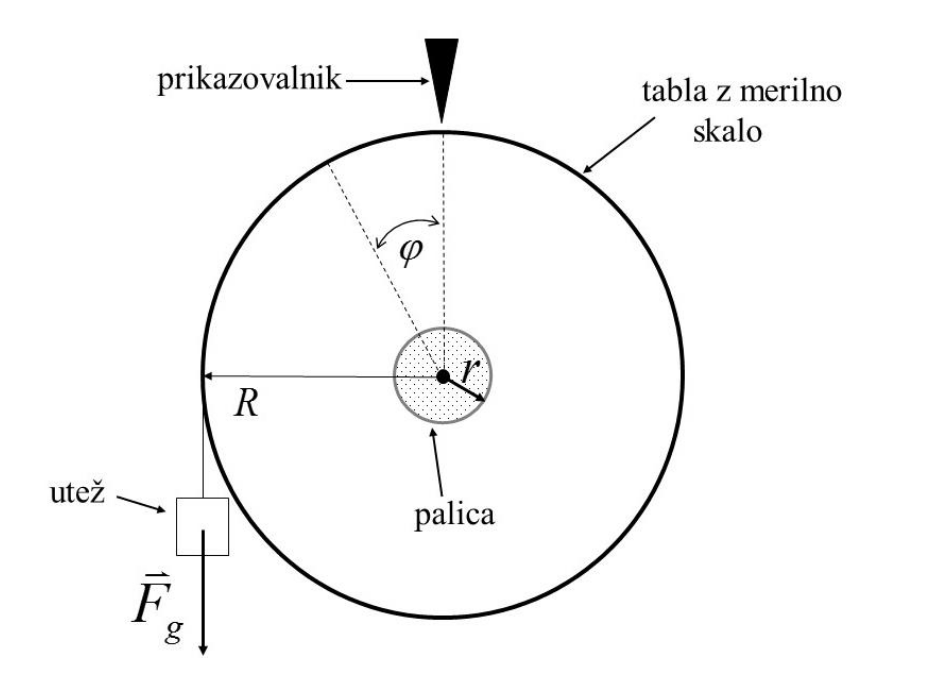
\includegraphics[width=0.9\textwidth]{skica1}
        \caption{Skica eksperimenta}
        \label{fig:1}
    \end{figure}
    Izmerjen polmer kolesa:
    \begin{align*}
        R = (11,4 \pm 0.1) cm \\
    \end{align*}
    Vsaka utež je torej ustvarjala navor $M = 0.0114 Nm$

    Spodaj so tabele meritev opravljene za vsako palico:
    ($\phi_1$ in $\phi_2$ sta meritvi v obe smeri, da lahko vemo da ni prišlo do plastičnih deformaciji ali zdrsa oprijema, $\delta \phi$ pa je relativni zasuk.)

    \subsection{Palica 1 - baker}

    \begin{align*}
        L_1 = (46,6 \pm 0,1)cm
        r_1 = (0,99 pm 0,01) mm
    \end{align*}

    \begin{table}[H]
        \centering
        \begin{tabular}{|c|c|c|c|c|}
            \hline
            $F$ [N] & M [Nm] & $\phi_1$ [$^\circ$] & $\phi_2 [^\circ]$ & $  \phi [^\circ]$\\
            \hline
            0.0  & 0.011 & 36  & 34  & 0 \\
            0.1  & 0.022 & 31  & 27  & 5 \\
            0.2  & 0.034 & 25  & 21  & 11 \\
            0.3  & 0.045 & 19  & 16  & 17 \\
            0.4  & 0.050 & 13  & 11  & 23 \\
            0.5  & 0.068 & 7   &  7  & 29 \\
            \hline
        \end{tabular}
        \caption{tabela baker}
        \label{tab:baker}
    \end{table}

    \subsection{Palica 2 - medenina}
    \[
        L_2 = (49,3 \pm 0,1) cm
        r_2 = (0,99 \pm 0,01) mm
    \]
    \begin{table}[H]
        \centering
        \begin{tabular}{|c|c|c|c|c|}
            \hline
            $F$ [N] & M [Nm] & $\phi_1$ [$^\circ$] & $\phi_2 [^\circ]$ & $  \phi [^\circ]$\\
            \hline
            0.0  & 0.011 & 61  & 59  & 0 \\
            0.1  & 0.022 & 56  & 53  & 5 \\
            0.2  & 0.034 & 51  & 48  & 11 \\
            0.3  & 0.045 & 46  & 43  & 16 \\
            0.4  & 0.050 & 40  & 38  & 21 \\
            0.5  & 0.068 & 34  & 34  & 26 \\
            \hline
        \end{tabular}
        \caption{tabela medenina}
        \label{tab:medenina}
    \end{table}

    \subsection{Palica 3 - aluminij}
    \[
        L_2 = (48,4 \pm 0,1) cm
        r_2 = (0,99 \pm 0,01) mm
    \]
    \begin{table}[H]
        \centering
        \begin{tabular}{|c|c|c|c|c|}
            \hline
            $F$ [N] & M [Nm] & $\phi_1$ [$^\circ$] & $\phi_2 [^\circ]$ & $  \phi [^\circ]$\\
            \hline
            0.0  & 0.011 & 80  & 80 & 0 \\
            0.1  & 0.022 & 77  & 77 & 3 \\
            0.2  & 0.034 & 74  & 74 & 6 \\
            0.3  & 0.045 & 71  & 70 & 10 \\
            0.4  & 0.050 & 67  & 67 & 13 \\
            0.5  & 0.068 & 64  & 64 & 16 \\
            \hline
        \end{tabular}
        \caption{tabela aluminij}
        \label{tab:aluminij}
    \end{table}

    \subsection{Palica 4 - jeklo/železo}
    \[
        L_2 = (48,4 \pm 0,1) cm
        r_2 = (0,99 \pm 0,01) mm
    \]
    \begin{table}[H]
        \centering
        \begin{tabular}{|c|c|c|c|c|}
            \hline
            $F$ [N] & M [Nm] & $\phi_1$ [$^\circ$] & $\phi_2 [^\circ]$ & $  \phi [^\circ]$\\
            \hline
            0.0  & 0.011 & 42  & 40 & 0 \\
            0.1  & 0.022 & 35  & 34 & 7 \\
            0.2  & 0.034 & 32  & 31 & 10 \\
            0.3  & 0.045 & 28  & 27 & 14 \\
            0.4  & 0.050 & 24  & 24 & 17 \\
            0.5  & 0.068 & 21  & 21 & 20 \\
            \hline
        \end{tabular}
        \caption{tabela jeklo/železo}
        \label{tab:jeklo/železo}
    \end{table}

    \section{Grafi in rezultati}
    Spodaj so prikazani grafi in linearni "fit-i".
    Fitali smo enačbo:
    \[
        M = \gamma \phi
    \]
    Da smo lahko vstavili v:
    \[
        \gamma =  \frac{\pi r^4 G}{2 L}
    \]
    In izrazli G (strižni modul snovi):
    \[
        G = \frac{\gamma 2 L }{\pi r^4}
    \]

    Gremo to naredit za vsako palico in ugotovit strižni modul vsake.
    (na grafih je oznaka k je konstantni člen oziroma $\gamma$)
    \subsection{Palica 1 - baker}

    \begin{figure}[H]
        \centering
        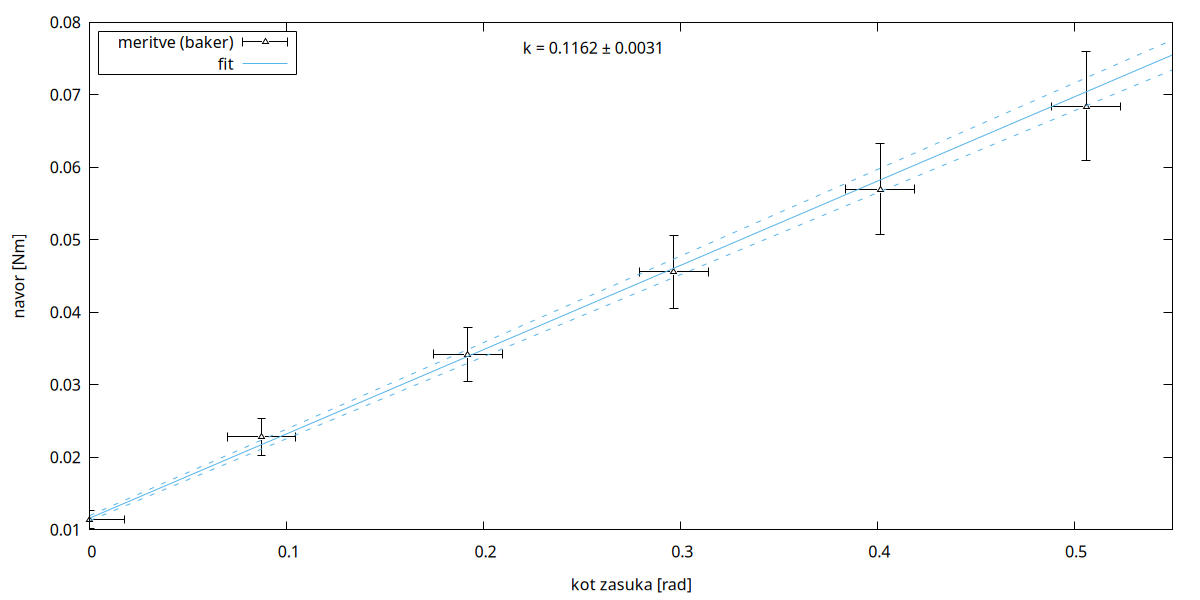
\includegraphics[width=0.9\textwidth]{baker}
        \caption{Graf 1}
        \label{fig:2}
    \end{figure}
    \[
        \gamma = (0,116 \pm 0,003) Nm
    \]
    Sledi:
    \[
        G = (36 \pm 4) 10^9 \frac{N}{m^2}
    \]
    \subsection{Palica 2 - medenina}

    \begin{figure}[H]
        \centering
        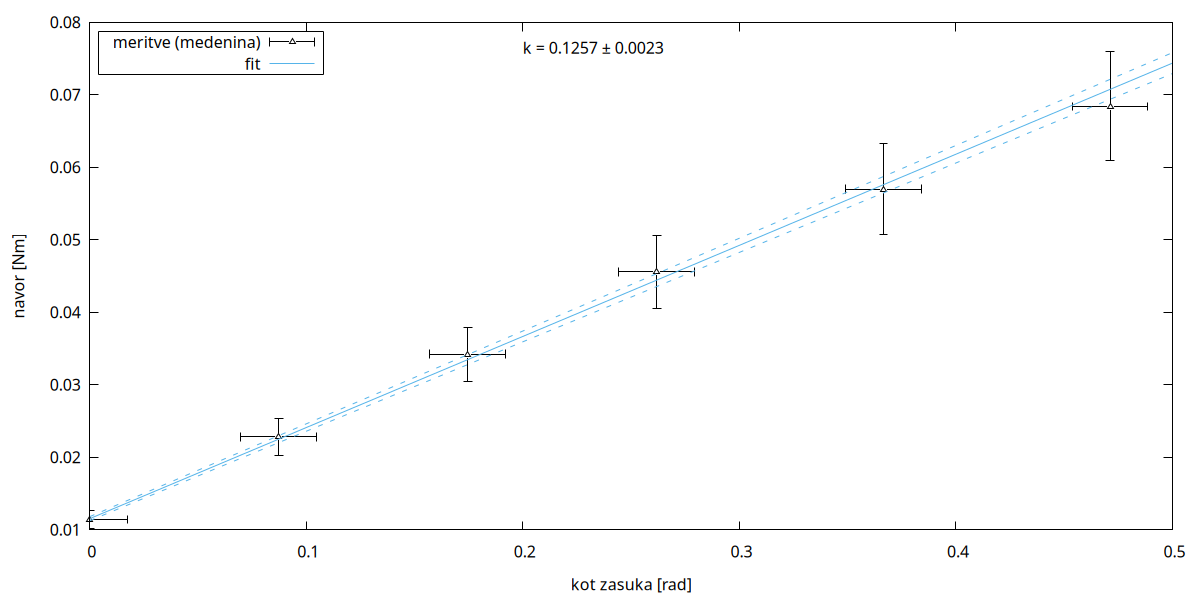
\includegraphics[width=0.9\textwidth]{medenina}
        \caption{Graf 2}
        \label{fig:3}
    \end{figure}
    \[
        \gamma = (0,126 \pm 0,002) Nm
    \]
    Sledi:
    \[
        G = (39 \pm 3) 10^9 \frac{N}{m^2}
    \]
    \subsection{Palica 3 - aluminij}

    \begin{figure}[H]
        \centering
        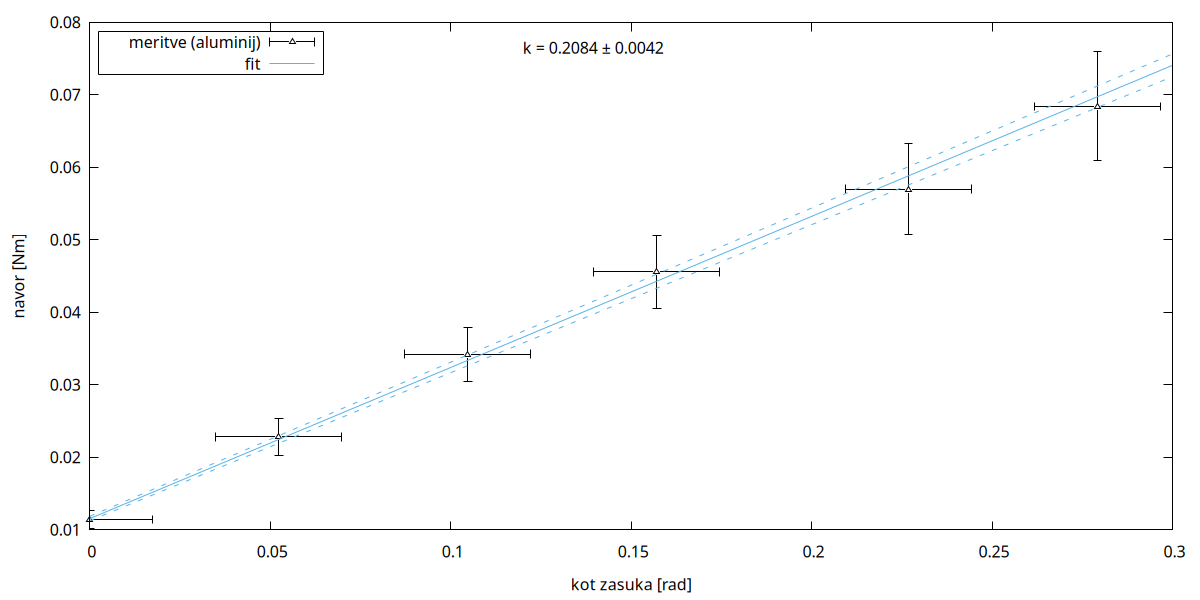
\includegraphics[width=0.9\textwidth]{aluminij}
        \caption{Graf 3}
        \label{fig:4}
    \end{figure}
    \[
        \gamma = (0,208 \pm 0,004) Nm
    \]
    Sledi:
    \[
        G = (27 \pm 2) 10^9 \frac{N}{m^2}
    \]
    \subsection{Palica 4 - jeklo/železo}

    \begin{figure}[H]
        \centering
        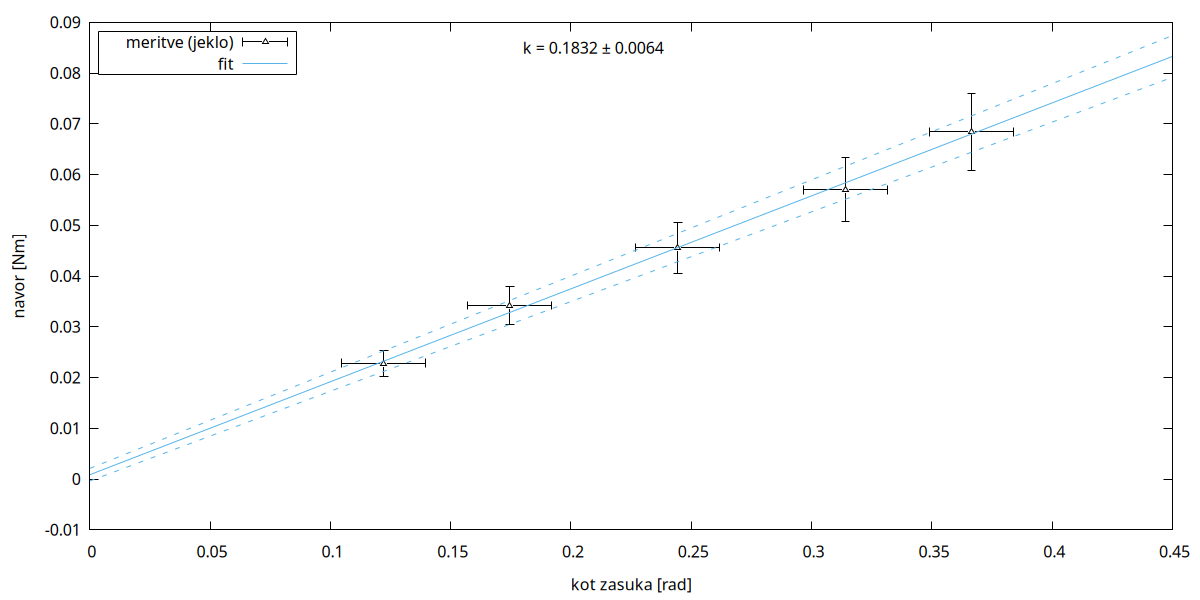
\includegraphics[width=0.9\textwidth]{jeklo}
        \caption{Graf 4}
        \label{fig:5}
    \end{figure}
    \[
        \gamma = (0,183 \pm 0,004) Nm
    \]
    Sledi:
    \[
        G = (57 \pm 5) 10^9 \frac{N}{m^2}
    \]


    \section{odgovori na vprašanja}
    \textit Izpeljava enačbe 2)

    Iz literature ($\tau - strizna napetost$):
    \[
        \tau = \frac{F}{S} = G \frac{\Delta x}{L} =  G \frac{r \phi}{L}
    \]
    Zapisemo defirencialno malo:
    \[
        F = \tau S,
        dF = \tau dS
    \]
    Navor je:
    \[
        dM = r dF
    \]
    Vsavimo dF:
    \[
        dM = r \tau dS
    \]
    Iz začetka vstavimo:
    \[
        dM = r (G \frac{r \phi}{L}) dS
    \]
    Integral...
    \[
        M = \frac{G \phi}{L} \int_{S1}^{S2} r^2 dS
    \]
    Integral, ki ostane je definicija vstrajnostnega momenta.
    \[
        M = \frac{G \phi}{L} J = \gamma \phi
    \]
    Vstrajnosti moment palice je:
    \[
        J_{palica} = \frac{\pi r^4}{2}
    \]
    Vstavimo in dobimo:
    \[
        G = \frac{2 \gamma L}{\pi r^4}
    \]



\end{document}